

\chapter[A Global Reflection: The Great Lakes and Water Insecurity]{A Global Reflection:\\The Great Lakes and Water Insecurity}
\label{cp:global-reflection}

\vspace{.935em}

The Great Lakes (\autoref{fig:great-lake}), comprising five large bodies of freshwater — Superior, Michigan, Huron, Erie, and Ontario—form the largest surface freshwater system on Earth, accounting for approximately 20\% of the world's total supply \autocite{canada2025greatlakes}. Situated on the border between
Canada and the United States, they play a critical role in supporting biodiversity, regional economies, and drinking water supplies. However, these vital water resources are increasingly threatened by both environmental and anthropogenic factors \autocite{looby2022compact}. These challenges not only compromise the ecological health of the lakes but also reflect broader global concerns about water security. Several key factors contribute to the escalating risks facing this essential freshwater system: 

\begin{figure}[htpb]
    \centering
    \fbox{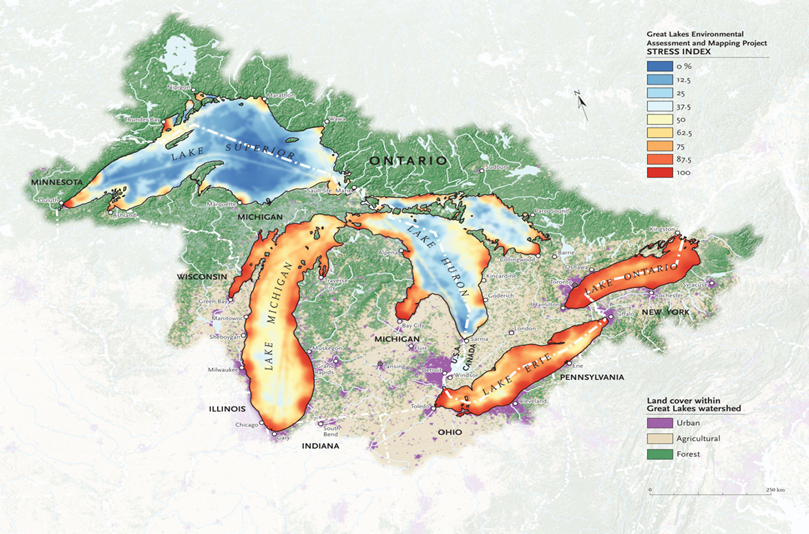
\includegraphics[width=\linewidth]{Figures/The Great Lakes.png}}
    \caption{The Great Lakes}
    \label{fig:great-lake}
\end{figure}

\section{Drought and Water Diversion Pressures}
Persistent droughts in the western United States have renewed interest in diverting Great Lakes water to support agricultural and municipal demands. Although the Great Lakes Compact (2008) prohibits most diversions, the approval of Waukesha, Wisconsin’s request under a special exemption has raised concerns \autocite{wisconsin2025waukesha}\autocite{walker2025mapping}. This decision could establish a precedent for future diversion claims, particularly as climate change intensifies drought severity across North America.

\section{Invasive Species Disruption}
Over 200 invasive species, including goby fishes, zebra and quagga mussels (see \autoref{cp:invasive-species}), have been introduced to the Great Lakes through ballast water discharge (as seen in \autoref{cp:ballast}) from international shipping \autocite{bongiorno2025invasion}. These species alter nutrient cycles, outcompete native fauna, and destabilize food webs, leading to ecological imbalances that affect water quality and biodiversity. Their continued spread presents significant management challenges for maintaining ecosystem resilience.


\section{Avian Botulism and Wildlife Health}
Shifts in water chemistry and food web dynamics, driven by invasive species and algal blooms, have created favorable conditions for avian botulism outbreaks \autocite{bongiorno2025invasion}. The botulinum toxin accumulates in fish and waterfowl, resulting in widespread bird mortality each year and further threatening the region’s vulnerable wildlife. This phenomenon underscores the complex and cascading impacts of ecosystem disruption caused by human activities.

\section{Climate Change and Extreme Weather Events}
Rising temperatures are altering thermal dynamics in the Great Lakes, leading to reduced ice cover, increased evaporation, and more frequent water level fluctuations \autocite{mishra2011thermal}. These changes contribute to heavier precipitation events, flooding, and shoreline erosion, stressing infrastructure and ecosystems alike. Climate-induced variability adds to the difficulty of maintaining water quality and sustainable lake management.

The struggles of the Great Lakes highlight the global water security crisis, where invasive species, climate change, and conflicts over water access intersect. Similar patterns are observed
in other large freshwater systems worldwide, driven by transboundary pollution, shipping practices, and increasing demand for limited water resources \autocite{un2021progress}. The experience of the Great Lakes emphasizes the need for proactive governance, international cooperation, and the integration of ecological sustainability into freshwater policy planning.
